\documentclass[12pt]{article}

\usepackage[utf8]{inputenc}
\usepackage[spanish]{babel}
\usepackage{times}
\usepackage{amssymb}
\usepackage{graphicx}
\usepackage{enumerate}
\usepackage[left=3.5cm,top=3.0cm,bottom=2.0cm,right=2.0cm]{geometry}
\title{Sistema de Control de Versiones}
\author{Yerson Coaquira Calizaya}

\begin{document}
\maketitle
\section{Introducción}
Este es un pequeño trabajo de investigación para el curso de Base de Datos II.
Básicamente el trabajo consta de tres partes: Los objetivos, el Marco Teórico y las Conclusiones. 

\section{Marco Teórico}

\subsection{El SCV}
Un sistema de control de versiones es una herramienta que registra todos los cambios hechos en uno o más proyectos, guardando así versiones del producto en todas sus fases del desarrollo. Las versiones son como fotografías que registran su estado en ese momento del tiempo y se van guardando a medida que se hacen modificaciones al código fuente. \newline
Un sistema de control de versiones debe proporcionar:
\begin{itemize}
	\item[$*$] Mecanismo de almacenamiento de los elementos que deba gestionar.
	\item[$*$] Posibilidad de realizar cambios sobre los elementos almacenados (ej. modificaciones parciales, añadir, borrar, renombrar o mover elementos).
	\item[$*$] Registro histórico de las acciones realizadas con cada elemento o conjunto de elementos (normalmente pudiendo volver o extraer un estado anterior del producto).
\end{itemize}

En los principales tipos de SCV tenemos en las siguientes gráficas:


\begin{figure}
\begin{center}
  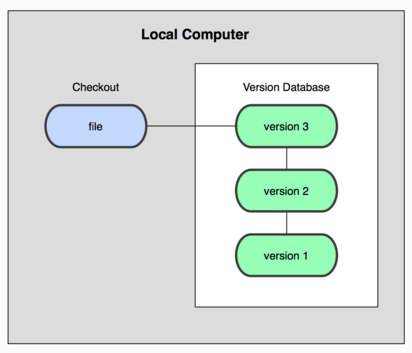
\includegraphics[width=0.35\textwidth]{imagenes/grafico1.png}
\caption{Sistemas de Control de Versiones Locales}

  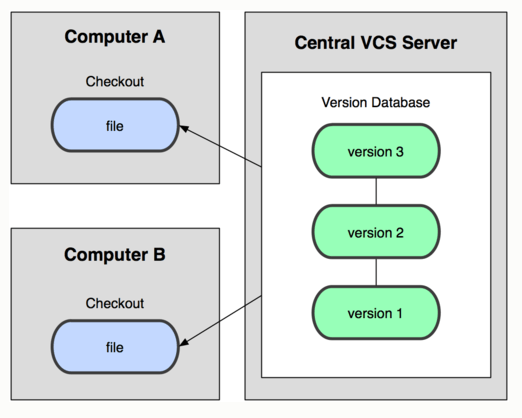
\includegraphics[width=0.35\textwidth]{imagenes/grafico2.png}
\caption{Sistemas de Control de Versiones Centralizados}

  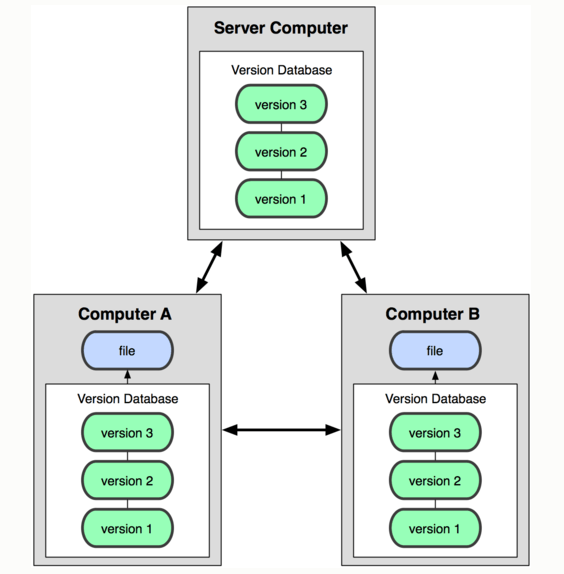
\includegraphics[width=0.35\textwidth]{imagenes/grafico3.png}
\caption{Sistemas de Control de Versiones Distribuidos}
\end{center}
\end{figure}

\newpage
\subsection{El Git}
Es un software para controlar versiones de nuestras aplicaciones, ejem: Estamos realizando un ERP y queremos compartirlo entre todos los desarrolladores de nuestro equipo para que los cambios que hagan puedan ser sincronizados en uno solo.

\subsubsection{GitHub}
Es un host para Git que nos permite almacenar proyectos open sources. Es decir que los proyectos que alojemos van a ser públicos, esto es ideal para compartir código con otros y generar colaboración entre los demás para dar mejoras a los proyectos que se publiquen.Podemos tener un repositorio privado pero tiene un costo.
\ \
El funcionamiento es fácil:
\begin{itemize}
	\item[$*$]Lo primero que debemos hacer es crear una cuenta en https://github.com. La activamos por mail y ya podemos crear nuestros repositorios. Los repositorios de Github son el almacén que utilizamos para guardar nuestro código. 
\item[$*$]Github nos ofrece la opción de crear un repositorio vacío, recomendable cuando vamos a iniciar un nuevo desarrollo, o la opción de importar un proyecto ya existente, elegimos la que más nos convenga y mediante unos pocos comandos de consola configuramos la rama principal de nuestro repositorio, que por defecto se llamará "master". 
\item[$*$]Cada programador puede crear sus propias ramas de desarrollo, donde tiene que llevar a cabo sus modificaciones, sin interferir en el trabajo de sus compañeros. Cuando terminamos y validamos un desarrollo paralelo, lo unimos con la rama principal y todos los miembros del equipo pueden descargar las nuevas modificaciones, sin alterar los desarrollos que estén llevando cabo en ese momento. 
\item[$*$] Después de alojar el repositorio público en Github.com, cualquier usuario de la comunidad podrá aportar ideas, hacer un seguimiento del proyecto, incluso copiarlo y modificarlo a su gusto bajo la misma licencia.
\end{itemize}

\begin{figure}
\begin{center}
  
\includegraphics[width=0.4\textwidth]{imagenes/github.png}
\end{center}
\end{figure}

\newpage
\subsection{El VSTS}
El Visual Studio Team Servicies es un servicio que ofrece Microsoft para organizar nuestro proyecto, usemos o no el IDE Visual Studio, que nos puede ser útil.
\begin{itemize}
\item[$*$] Puede compilar windows, IOS, Android, Java, LInux y Xamarin.
\item[$*$] Usa su DLS habitual.
\item[$*$] Prueba y publica sus apps.
\end{itemize}

Ademas de eso también es de fácil personalización como:
\begin{itemize}
\item[$*$]Los procesos son editables a través de la Web.
\item[$*$]No hay que trabajar con XAML.
\item[$*$]Permite usar conocimientos de script.
\end{itemize}

\begin{figure}
\begin{center}
  
\includegraphics[width=0.4\textwidth]{imagenes/vsts.png}
\end{center}
\end{figure}

\end{document}
